
\begin{figure*}[t!]
  \centering
  \begin{minipage}[b][10cm][t]{0.32\linewidth}
    \centering
    \captionsetup{justification=centering}   
    \begin{minted}[xleftmargin=1em,linenos,autogobble,tabsize=2,framesep=1pt,frame=single,fontfamily=courier,fontsize=\fontsize{7}{8}\selectfont,highlightlines={10-14}]{scala}
			import DFiant._
			
			trait MA4 extends DFDesign {
				val a    = DFSInt[16] <> IN init 0
				val b    = DFSInt[16] <> IN init 0
				val c    = DFSInt[16] <> IN init 0
				val d    = DFSInt[16] <> IN init 0
				val o    = DFSInt[16] <> OUT
				
				def ma(src: DFSInt[16]) = {     
					val acc = DFSInt[18] init 0    
					acc := acc - src.prev(4) + src 
					(acc / 4).toWidth(16)
				}
				def avg2(
				  src1: DFSInt[16], 
				  src2: DFSInt[16]
				)=((src1 +^ src2) / 2)
				  .toWidth(16)
					//  (_ +^ _)=with-carry addition
					
				o := avg2(
					avg2(ma(a), ma(b)), 
					avg2(ma(c), ma(d))
				)
			}
			
			
			
			
			
			object MA4App 
			extends DFApp.VHDLCompiler[MA4]
    \end{minted}
    \subcaption{The MA4 DFiant code is concise and portable}
    \label{fig:MADFiant}
  \end{minipage}%
  \hfill
  \begin{minipage}[b][10cm][t]{0.325\linewidth}
    \centering
    \captionsetup{justification=centering}
		\begin{minted}[xleftmargin=1em,autogobble,tabsize=2,framesep=1pt,frame=single,fontfamily=courier,fontsize=\fontsize{7}{8}\selectfont,highlightlines={1-33}]{vhdl}
			...
			signal acc      :signed(17 downto 0);
			signal acc_prev1:signed(17 downto 0);
			signal src_prev1:signed(15 downto 0);
			signal src_prev2:signed(15 downto 0);
			signal src_prev3:signed(15 downto 0);
			signal src_prev4:signed(15 downto 0);
			...
			sync_proc : process (CLK, RSTn)
			begin
			  if RSTn = '0' then
			    acc_prev1   <= 18d"0";
			    src_prev1   <= 16d"0";
			    src_prev2   <= 16d"0";
			    src_prev3   <= 16d"0";
			    src_prev4   <= 16d"0";
			  elsif rising_edge(CLK) then
			    acc_prev1   <= acc;
			    src_prev1   <= src;
			    src_prev2   <= src_prev1;
			    src_prev3   <= src_prev2;
			    src_prev4   <= src_prev3;
			  end if;
			end process sync_proc;
			...
			async_proc : process (all)
			  variable v_acc:signed(17 downto 0);
			begin
			  v_acc := acc_prev1;
				v_acc := v_acc - src_prev4 + src;
			  acc   <= v_acc;
			  ma    <= resize(acc sra 2, 16)
			end process async_proc;
    \end{minted}
    \subcaption{
			DFiant code lines 11-13 compiled to VHDL
		}
%    \captionof{figure}{
%    	The MA4 DFiant lines 11-12 compiled to VHDL \\ 
%    	The DFiant code is extremely compact in comparison.
%    }
    \label{fig:MAVHDL}
  \end{minipage}%
	\hfill
  \begin{minipage}[b][10cm][t]{0.34\linewidth}
		\centering

  	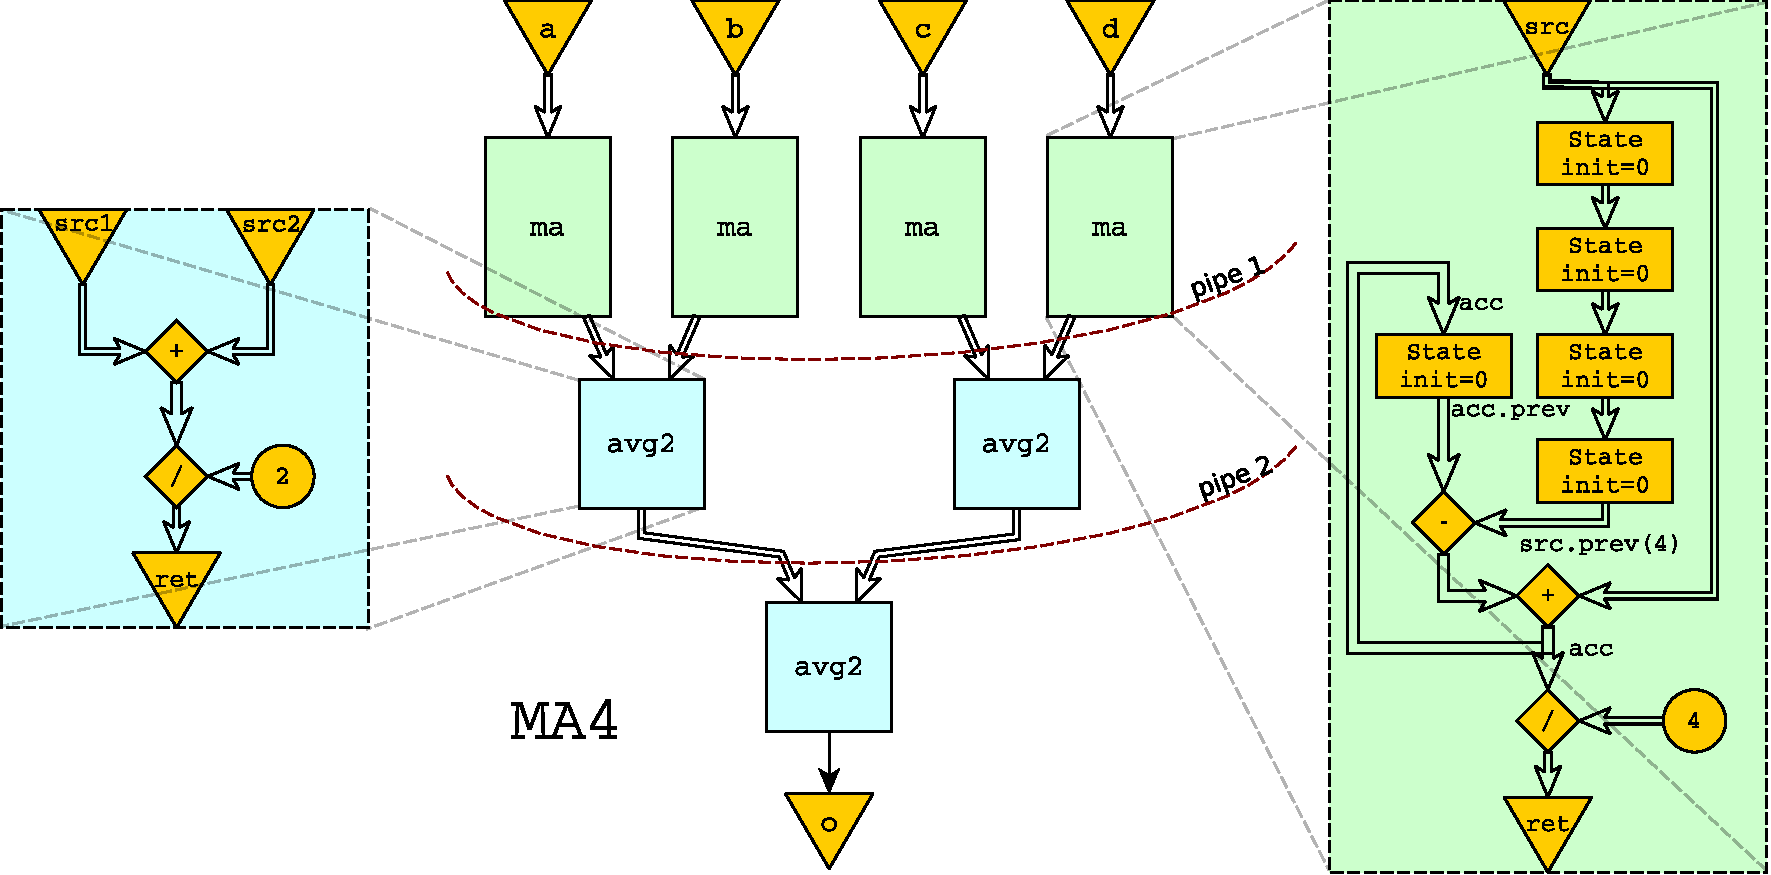
\includegraphics[width=0.884\linewidth]{graphics/ma.pdf}
  	\captionsetup{justification=centering}
    \subcaption{
			The MA4 dataflow graph
		}
		\label{fig:MADraw}
  \end{minipage}%
  \captionsetup{justification=centering}      
  \caption{
		Our MA4 implementation (the inputs are \code{a}, \code{b}, \code{c}, \code{d} and the output is \code{o}) \\ 
		The entire design is a composition of the \code{ma} and \code{avg} functions (detailed blowouts are depicted as well). \\ 
		The compiler places pipeline tags to achieve the required performance and the backend inserts registers accordingly. \\
		The concurrent construction is implied from independent sequential compositions thanks to the dataflow abstraction. 
	}
\end{figure*}

\section{The DFiant Language Overview}
\label{sec:dfiant}
DFiant is a Scala library and thus possesses various rich type safe language constructs. DFiant also incorporates unique language semantics, as expected from a DF-HDL. Throughout this section we elaborate on these constructs and semantics via our running example, a four-by-four moving average (MA4) unit. The MA4 has four 16-bit integer input channels and is required to output the average of all channels, while each channel is averaged by a four-sample moving window continuously. The complete MA4 DFiant implementation and its dataflow graph are available in \fig{fig:MADFiant} and \ref{fig:MADraw}, respectively. \fig{fig:MAVHDL} presents a subset of the DFiant-generated VHDL (2008) code derived from lines 11--13 in \fig{fig:MADFiant}.


\subsection{Hello DFiant World!}
The DFiant code in \fig{fig:MADFiant} demonstrates the structure of any DFiant program: it imports the \code{DFiant} library (line 1), creates the top-level design by extending the \code{DFDesign} abstract class (lines 3--26), and creates a runnable application that instantiates the top design trait, and compiles it into a VHDL file (linees 32--33).

The MA4 design is fairly straightforward. Lines 4--8 generate the signed dataflow ports and include a \code{0} value initialization (see Section~\ref{sec:state_constructs}). 
Lines 10--14 define the function \code{ma} that generates a single four-sample moving average, while lines 15--19 define the function \code{avg2} that generates a two-input average unit. Finally, lines 22--25 compose \code{avg2} and \code{ma} to generate the entire MA4 functionality and assign it to the output port \code{o}. We elaborate on the unique DFiant constructs and semantics in the next sections.


\subsection{Dataflow Variable Semantics}
DFiant code is expressed in a sequential manner yet employs an asynchronous dataflow programming model to enable an intuitive concurrent hardware description. For this purpose, DFiant applies the following rules:

\subsubsection{Concurrency and Execution Order} 
Concurrency is implicit and the data scheduling order, or \textit{token-flow}, is set by the \textit{data dependency}. DFiant schedules all independent dataflow expressions concurrently, while dependent operations are synthesized into a guarded FIFO-styled pipeline. The MA4 dataflow graph in \fig{fig:MADraw} demonstrates the concurrent paths constructed from the dataflow dependency. 

\subsubsection{Basic Operations} 
\label{sec:basic_ops}
Each application of an arithmetic/logic operator is translated into the appropriate hardware construction and applies a dataflow \emph{join} on their arguments. The arguments require a valid token for consumption to produce a new token generated from the operations. For example, \code{+} in \code{avg2} joins \code{src1} and \code{src2} and requires a token from both to produce the token \code{src1 + src2}.

\subsubsection{Path Divergence} 
\label{sec:path_div}
Diverging paths are implicitly \emph{forked}, so token production is possible if all target nodes are ready to consume the token. For example, \code{acc} result in \code{ma} is forked into a division operation and the state feedback.	It is impossible to consume an invalid token and once a token is consumed it is invalidated.

\subsubsection{Constants} 
Any Scala primitive value is considered as a constant when applied as an argument to a dataflow operation. For example, the value \code{2} in \code{avg2} is a primitive \code{Int} and is considered a constant in the division operation. Semantically, a constant is an infinite token generator that produces a new token with the same initial value each time the token is consumed.

\subsubsection{Pruning}
Unused nodes always consume tokens and are discarded during compilation. 

\subsubsection{Bit-Accurate Operations and Type Inference}
DFiant supports various basic dataflow types such as \code{DFBool}, \code{DFBits}, and others.
All DFiant's dataflow types are bit-accurate and structurally static, with their bit-width set upon construction (e.g., at line 11 of \code{MA4} the variable \code{acc} is an 18-bit signed integer). Operations between dataflow variables produce a bit-accurate result with the proper type inference. For example, at line 12 of \code{MA4}, a 16-bit value is subtracted from an 18-bit value which results in an 18-bit value. In line 18 the with-carry addition between \code{src1} and \code{src2} returns a carried 17-bit. DFiant also employs various type-safe restrictions to protect designers from unexpected or surprising behavior (e.g., it is unclear what should occur at \code{DFUInt[4] - 1000}).

\subsubsection{Assignment and Mutability}
\label{sec:mutability}
DFiant supports dataflow variable "mutation" via the \code{:=} operator. This not an actual mutation but only a change of the variable reference to a different dataflow stream (hardware \emph{construction} is immutable). Assignments are also used inside conditional constructs (\sect{sec:conditional}) and to set the input of a feedback state (\sect{sec:state_update}).

Dataflow variables can be either mutable (accept \code{:=}) or immutable (compiler error for \code{:=}). The mutability trait depends on the type and sometimes also on the context within it is applied. For example, we cannot assign to a the dataflow stream returned at line 13 of \code{MA4}. The only mutable variables are the ones explicitly constructed or output ports as seen at lines 11 and 8 of \code{MA4}. Mutation must be local to the context of assignment operation (e.g., cannot assign to variable outside its design).
Note: do not confuse with Scala-level mutation which is enabled by using \code{\textbf{var}} instead of \code{\textbf{val}} (the DFiant compiler disallows constructing DFiant objects under a \code{\textbf{var}} reference). 

\subsubsection{Read Access}
All dataflow values can be read (yes, even output ports). The only exception exist in an output port that is neither assigned or initialized because in this situation the reader will only consume stall bubble tokens and possibly lead to a system deadlock.

\subsubsection{Bit Aliasing and Casting} 
In general, aliasing is a mechanism to reference a cluster of one or more dataflow variable parts and cast it to any dataflow variable type that has the same bit width. The most trivial aliasing construct is \code{.bits(hi, lo)} that selects part of any dataflow variable from bit \code{hi} downto to bit \code{lo} and casts it to a bit vector. The aliasing mechanism implements bit concatenation, selection, shifting, reversal, and inversion. Aliasing preserves the mutability property: an alias of an immutable variable is immutable, while an alias of a mutable variable is mutable. Mutating an alias is equivalent to mutating the original aliased variable(s) at the relevant bit indexes. Aliasing of an alias is also possible, while maintaining relative bits indexing.  

%
%Fig.~\ref{fig:Aliasing} demonstrates aliasing code and its effect on the contents of a dataflow variable (\code{bits128}). Each line code does as follows:
%\begin{enumerate}
%  \item Constructs a new 128-bit vector, \code{bits128}, and clears it.
%  \item Creates a new alias, \code{alias64}, which references the most significant 64 bits of \code{bits128}. Since \code{bits128} is a \code{DFBits} variable, there is no need to invoke \code{.bits()}, and we can apply the required indexes directly.
%  \item Creates a new alias, \code{alias32}, which references the least significant 32 bits of \code{alias64}, which reference bits 64 to 95 of \code{bits128}.
%  \item Constructs a new double precision floating point dataflow variable, \code{dbl}, and initialize its value as \code{1.0} (hexadecimal value of \code{0x3FF00...0}).
%  \item Modifies the least significant byte of \code{dbl}.
%  \item Sets the most significant bit of \code{bits128}.
%  \item Assigns \code{dbl} to the least significant 64 bits of \code{bits128} through casting. All the bits of \code{dbl} are selected because \code{.bits()} is invoked without index parameters.
%  \item Modifies a byte of \code{bits128}.
%  
%\end{enumerate}
%
%\begin{figure}[h]
%  \centering
%  \begin{minipage}[b][3cm][b]{0.57\linewidth}
%    \vfill
%    \begin{minted}[xleftmargin=1.5em,linenos,autogobble,tabsize=2,framesep=1pt, frame=single,fontsize=\fontsize{8}{8}\selectfont]{scala}
%    val bits128 = DFBits[128] := 0
%    val alias64 = bits128(127, 64)
%    val alias32 = alias64(31, 0)
%    val dbl = DFDouble() := 1.0
%    dbl.bits(7,0) := 0x28
%    bits128(127) := 1
%    bits128(63, 0) := dbl.bits()
%    alias32(16, 8) := 0x57		    
%    \end{minted}
%    \vfill
%    \subcaption{DFiant code}
%  \end{minipage}%
%  \hfill
%  \begin{minipage}[b][3cm][b]{0.42\linewidth}
%    \centering
%    \vfill
%    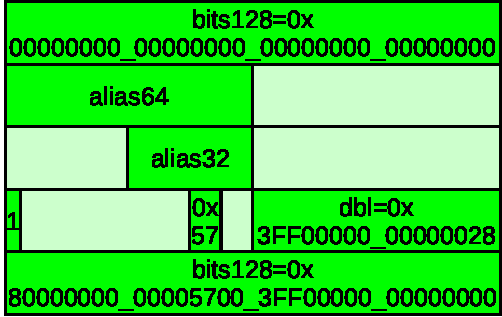
\includegraphics[width=\linewidth]{graphics/Aliasing.pdf} 
%    \vfill
%    \subcaption{Contents of \code{bits128}}
%  \end{minipage}
%  \captionof{figure}{Bit aliasing and casting example}
%  \label{fig:Aliasing}
%\end{figure}


\subsection{State Constructs and Semantics}
\label{sec:state_constructs}
In contrary to RTL languages, DFiant does not directly expose register and wire constructs. Instead, DFiant assumes every dataflow variable is a stream and provides constructs to initialize the token history via the \code{.init} construct, reuse tokens via the \code{.prev} construct, and update the state via the \code{:=} construct. Lines 11-12 in \fig{fig:MADFiant} along with their compiled VHDL representation in \fig{fig:MAVHDL} demonstrate the state semantics as follows:

\subsubsection{Initialization} The \code{.init} construct is accompanied by one or more token values and only sets the initial state history. For example, line 11 constructs a dataflow variable and initializes all of its history to zero value tokens. The history sequence is typed from left to right and sets tokens from newest to oldest, respectively. If the sequence is accessed beyond the oldest token then the oldest token is repeatedly produced. If the history is empty (not initialized) then stall bubble tokens are produced when accessed (see \sect{sec:stall_bubbles}). It is also possible to directly place bubble tokens in the history by writing either $\phi$ or \code{Bubble}.  

\subsubsection{History Access} The \code{.prev} construct reuses the previous state token. The very first "reused" token is the one set via \code{.init}. It is also possible to call \code{.prev(step)} with a step number argument to reuse older stream values. For any dataflow value \code{a} and a given positive integer \code{step}, a call to \code{a.prev(step)} is equivalent to repeated <step> applications of \code{a.prev.prev...prev}.
For example, in line 12 we reuse a \code{src} token from four steps ago. If the \code{src} token stream is "$1,2,3,4,...$" with a $0$ initialization, then the \code{src.prev(4)} token stream is "$0,0,0,0,1,2,3,...$".

\subsubsection{Distributive Property} The history access via \code{.prev} is distributive over all the basic DFiant operations. For example, the distributed \code{a.prev + b.prev} is equivalent to \code{(a + b).prev}. This means that the initialization history is also respectively affected from these basic operations.
 
\subsubsection{Stall Bubbles} 
\label{sec:stall_bubbles}
Invoking \code{.prev} on an uninitialized dataflow variable generates a stall bubble. Stall bubbles are consumed and produced like any other token, yet a basic operation with a stall bubble token must produce a stall bubble token. Additionally, stall bubbles do not affect a feedback state. The backend compiler is responsible to generate the additional logic required for existing design stalls. 

\subsubsection{State Update} 
\label{sec:state_update}
The new updated token is pushed into a dataflow stream by using the \code{:=} assignment operator. There can be more then one assignment to same variable, however only the last assignment updates the state and occurs when all dependent dataflow firing rules are satisfied. This rule is similar to signal update semantics in VHDL processes.

\subsubsection{Default Self-Generation} 
\label{sec:default_self_gen}
Any dataflow variable \code{a} has an implicit self-assignment \code{a := a.prev} that comes immediately after the variable construction. This creates an equivalent reference between \code{a} and \code{a.prev} which leads to a more intuitive programming.
For example, in line 12 we used \code{acc - ...} and not \code{acc.prev - ...}, since both expressions are equivalent.

\vspace{2ex}

Another example that illustrates the benefits of the DFiant state constructs is the 32-bit Fibonacci series generator in \fig{fig:FibGen}. The dataflow version is shorter than its VHDL counterpart~\cite{fibgenvhdl} and greatly resembles the formal Fibonacci definition: $F_0 = 0$, $F_1 = 1$, $F_n = F_{n-1} + F_{n-2}$ for $n > 1$. 

\begin{figure}[h]
  \centering
  \captionsetup{justification=centering}    

  \begin{minted}[xleftmargin=0.25\linewidth, xrightmargin=0.25\linewidth,frame=single,autogobble,linenos,tabsize=2,fontfamily=courier,fontsize=\fontsize{6}{7}\selectfont]{scala}
    trait FibGen extends DFDesign {
      val o = DFUInt[32] <> OUT
      val f = DFUInt[32] init (1, 0)
      f := f.prev + f.prev(2)
      o := f.prev(2) //output from 0
    }
  \end{minted}
  \captionof{figure}{A DFiant 32-bit Fibonacci series generator \\ Great resemblance to the formal Fibonacci definition}
  \label{fig:FibGen}
\end{figure}

Both \fig{fig:MAVHDL} and \fig{fig:FibGen} emphasize the advantages of DFiant state constructs over RTL registers and wires.
One advantage is that the DFiant code resembles its RTL counterparts, but is also very concise since state elements are automatically constructed when a stream history is accessed. Another advantage is portability, because state elements are not registers and therefore any type of state component is applicable. Our first synchronous backend indeed maps state elements to registers, but even an asynchronous backend can compile the same code and apply the Muller C-element~\cite{muller1957theory} as a state element. 

In comparison, many HLS tools rely on C and use \code{static} or global variables to define their explicit state. Indeed these variables abstract over registers, but their major disadvantage is that they prevent functional composition. For example, the \code{ma} function has a state and requires a static variable in its HLS implementation. This variable is shared among all \code{ma} function calls, so an HLS composition code similar to lines 22--25 of MA4 would not be possible as-is.

\subsection{Conditional Constructs and Semantics}
\label{sec:conditional}
DFiant has \code{ifdf} and \code{matchdf} conditional constructs which logically resemble the Scala \code{\textbf{if}} and \code{\textbf{match}}, respectively. These dataflow conditional constructs are also very similar to their RTL counterparts and yield multiplexer hardware. However, their semantics follow the same dataflow \emph{join} and \emph{fork} rules we described in Sections \ref{sec:basic_ops} and \ref{sec:path_div}, and therefore all dataflow values used within the conditional constructs are joined together and all modified dataflow variables which are referenced outside the conditional constructs are forked as well. Of course, if there is no need for this additional flow control logic, the default compiler yields a simple combinational structure.

\fig{fig:SeqDet} demonstrates a simple DFiant finite state-match (FSM) that utilizes these conditional constructs to detect the sequence "1001". The VHDL~\cite{seqdetvhdl} implementation is very similar but also a bit longer due to the split between the sequential and combination parts, which is applied automatically by the DFiant compiler.
Note we did not need to directly refer to \code{state.prev} at line 8, thanks to the default self generation described in \sect{sec:default_self_gen}.

\begin{figure}[t]
  \centering
  \captionsetup{justification=centering}    
  
  \begin{minted}[xleftmargin=0.18\linewidth, xrightmargin=0.18\linewidth,frame=single,autogobble,linenos,tabsize=2,fontfamily=courier,fontsize=\fontsize{6}{7}\selectfont]{scala}
    trait SeqDet extends DFDesign {
      val seqIn  = DFBool() <> IN
      val detOut = DFBool() <> OUT
      object State extends Enum.Auto {
        val S0, S1, S10, S100, S1001 = Entry
      }
      val state = DFEnum(State) init State.S0
      matchdf(state)
      .casedf(State.S0) {
        detOut := 0
        ifdf (seqIn) {state := State.S1}
        .elsedf      {state := State.S0}
      }.casedf(State.S1) {
        detOut := 0
        ifdf (seqIn) {state := State.S1}
        .elsedf      {state := State.S10}
      }.casedf(State.S10) {
        detOut := 0
        ifdf (seqIn) {state := State.S1}
        .elsedf      {state := State.S100}
      }.casedf(State.S100) {
        detOut := 0
        ifdf (seqIn) {state := State.S1001}
        .elsedf      {state := State.S0}
      }.casedf(State.S1001) {
        detOut := 1
        ifdf (seqIn) {state := State.S1}
        .elsedf      {state := State.S10}
      }
    }
  \end{minted}
  \captionof{figure}{A DFiant "1001" sequence detector FSM \\ Very similar to its VHDL counterpart}
  \label{fig:SeqDet}
\end{figure}



\subsection{Hierarchy and Connectivity}
So far, all examples demonstrated a single dataflow design without any hierarchies. The MA4 design managed to create structural encapsulations and composition via Scala definitions. Earlier, in \sect{sec:motivation}, we stressed the importance of any HDL to support hierarchies via constructs that describe components, ports and their connections. These DFiant features surpass the synthesizable capabilities of traditional HDLs, and are noticeably absent from HLS languages such as C++. 



\subsubsection{Dataflow IO Ports} 
\label{sec:io_ports}
Dataflow IO ports act in many ways just like dataflow variables. 
%The main difference is that only ports can be referenced outside the design in which they are constructed (this limitation may change in the future). 
Ports are used either to connect a parent design to its child or connect two child sibling designs. The operator \code{<>} is used both to construct dataflow ports (from dataflow variables) and create connections between ports. 
Dataflow ports can be either \code{IN} or \code{OUT} as seen at lines 7--8 of \code{MA4} and can also be initialized via \code{.init}. Input ports are immutable. Output ports are mutable, but only within the context of their owner design.  
There are various connectivity rules and semantic differences between a connection \code{<>} and an assignment \code{:=}.
%See \tbl{tbl:Box} for a brief comparison.

\subsubsection{Dataflow Designs} 
Dataflow designs are the basic hierarchy abstraction in DFiant. By extending the abstract class \code{DFDesign} the designer populates it with IO ports that makeup its interface and with dataflow variables and operations that makeup its implementation.
DFiant expands traditional structural composition capabilities by utilizing Scala's object oriented features such as inheritance and polymorphism, as well as finite loops and recursive composition. The hierarchical compositions provide the scope and dependencies for the dataflow variables. The difference between a Scala hierarchy and a DFiant hierarchy itself is that pure Scala constructs are transparent to the dataflow graph, as if the entire design is flattened, inlined, and unrolled. 

%\subsubsection{Dataflow Foldable Components (Grayboxes)}TBD

%\subsubsection{Realtime Components (Blackboxes)}
%Realtime components

%Figures \ref{fig:BoxTopCode}, \ref{fig:BoxTopDraw}, and \ref{fig:BoxTopTokens} showcase the flexibility when applying both DFiant hierarchies and Scala inheritance. Indeed these capabilities are no strangers to HL-RTLs such as Chisel, and may even be expressible by native RTLs in some cumbersome fashion, but all these languages still couple the design to its specific timing and target constraints. For example,  \code{NWParCross} should have larger PD than \code{NWPArDirect}. On the one hand, pipelining inside the \code{NWLeft} and \code{NWRight} may result in over-pipelining. while on the other hand, pipelining outside, in their parent designs, may cause the same. DFiant helps us describe a truly agnostic network and \emph{optionally} leave the hard work to the compiler. 
%Additionally, these figures highlight some of the differences between connections and assignments and how they affect the initialization throughout the design.

%\begin{table*}[t!]
  \small
  \begin{minipage}[t][9cm][t]{0.343\linewidth}
    \centering
    \captionsetup{justification=centering}
    \begin{minted}[xleftmargin=1em,linenos,autogobble,tabsize=2,framesep=1pt,frame=single,fontfamily=courier,fontsize=\fontsize{7}{8}\selectfont]{scala}
      //All networks have the same interface
      trait Network extends DFDesign {
        val iT = DFSInt[16] <> IN  //Top
        val iB = DFSInt[16] <> IN  //Bottom
        val oT = DFSInt[16] <> OUT //Top
        val oB = DFSInt[16] <> OUT //Bottom
      }
      //State in Top Connection
      trait NWLeft extends Network {
        iT.prev <> oT //Connection
        oB := iB + 5  //Assignment
      }
      //State in Bottom Assignment
      trait NWRight extends Network {
        iT <> oT * 3  //Connection
        oB := iB.prev //Assignment
      }
      //Parent box includes two sibling boxes
      trait NWParent extends Network {
        iT init (5, 7) //Initializing history
        iB init (2, 6) //Initializing history
        val nwL = new NWLeft {}
        val nwL = new NWRight {}
        nwL.iT <> iT
        nwL.iB <> iB
        nwR.oT <> oT
        nwR.oB <> oB
      }
      //Direct connections between siblings
      trait NWParDirect extends NWParent {
        nwL.oT <> nwR.iT
        nwL.oB <> nwR.iB
      }
      //Cross connections between siblings
      trait NWParCross extends NWParent {
        nwL.oT <> nwR.iB
        nwL.oB <> nwR.iT
      }
    \end{minted}
    \vfill
    \captionof{figure}{Various network designs \\ Featuring hierarchies and inheritance }
    \label{fig:BoxTopCode}
  \end{minipage}%
  \hfill
  \begin{minipage}[t][12cm][b]{0.64\linewidth}
    \centering
    \captionsetup{justification=centering}
    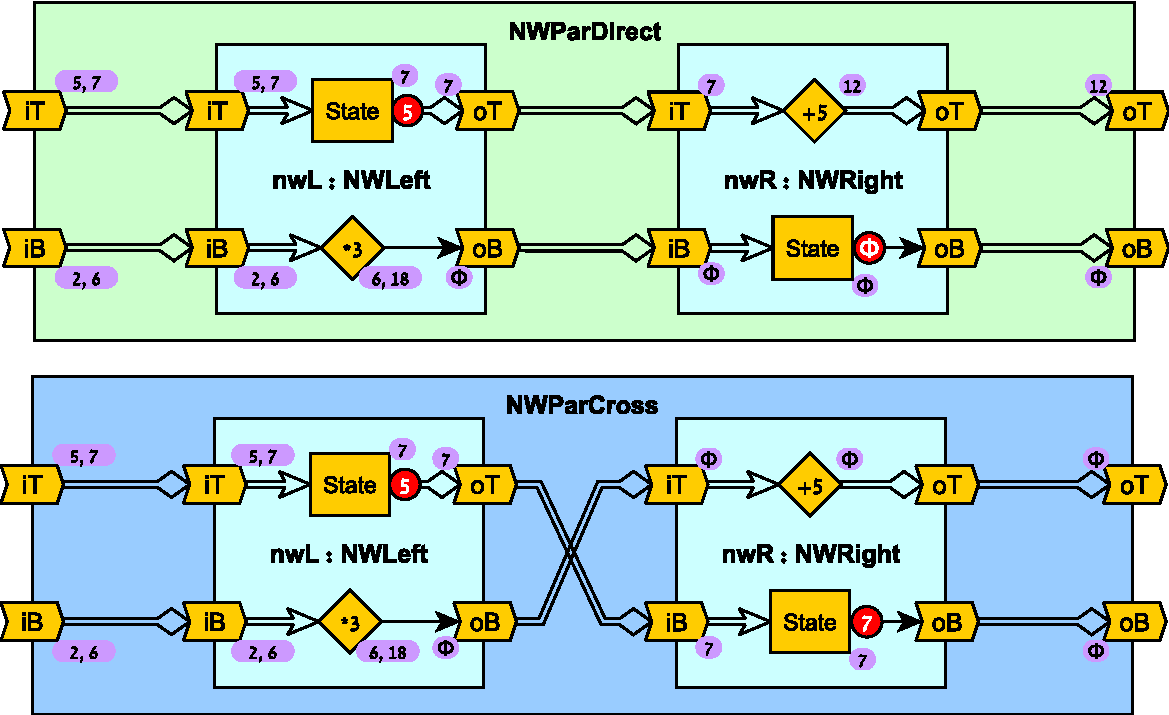
\includegraphics[width=0.9\linewidth]{graphics/connectivity.pdf}
    \captionof{figure}{
      Hierarichal drawing of \code{NWParDirect} and \code{NWParCross} \\
      The \colorbox{initcolor}{purple} numbers mark the initialization history as it is propagated according to the semantic rules of DFiant. The \colorbox{red}{\textcolor{white}{red}} numbers mark initial tokens generated by the state elements.
    }
    \vfill
    \label{fig:BoxTopDraw}
    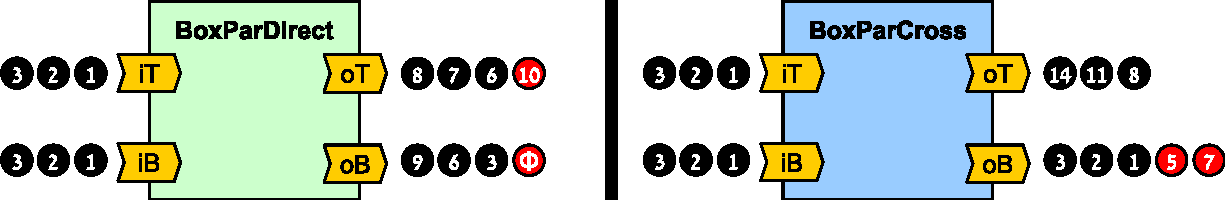
\includegraphics[width=0.9\linewidth]{graphics/connectivityTokens.pdf}
    \captionof{figure}{
      Input/Output token flow example to/from the two parent boxes (the rightmost tokens are the oldest). 
    }
    \label{fig:BoxTopTokens}
  \end{minipage}%
  \vspace{2ex}
  \hrule
  \vspace{2ex}
  \captionof{table}{Connection \code{<>} and Assignment \code{:=} Operator Comparison}
  \label{tbl:Box}
  \begin{tabular}{|c|c|c|}
    \hline 
    \textbf{Criteria} & \textbf{Connection \code{<>}} & \textbf{Assignment \code{:=}} \\ 
    \hline
    \begin{minipage}{0.1\textwidth}
      \flushleft
      Code
    \end{minipage} 
    &
    \begin{minipage}[c][1.5cm]{0.4\textwidth}
      \begin{minted}[autogobble,tabsize=2,framesep=1pt,fontfamily=pcr,fontsize=\fontsize{7}{8}\selectfont]{scala}
      trait IOConnection extends DFDesign {
        val i = DFUInt[8] <> IN
        val o = DFUInt[8] <> OUT
        o <> i
      }
      \end{minted}
    \end{minipage} 
    &  
    \begin{minipage}[c][1.5cm]{0.4\textwidth}
      \begin{minted}[autogobble,tabsize=2,framesep=1pt,fontfamily=pcr,fontsize=\fontsize{7}{8}\selectfont]{scala}
        trait IOAssignment extends DFDesign {
          val i = DFUInt[8] <> IN
          val o = DFUInt[8] <> OUT
          o := i
        }
      \end{minted}
    \end{minipage} 
    \\ 
    \hline 
    \begin{minipage}{0.1\textwidth}
      \flushleft
      Functional Diagram
    \end{minipage} 
    &
    \begin{minipage}[c][2cm]{0.10\textwidth}
      \centering
      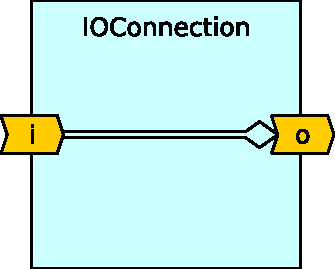
\includegraphics[height=1.8cm]{graphics/IOConnection.pdf}\\
    \end{minipage}%
    \hfill 
    \begin{minipage}[c][2cm]{0.27\textwidth}
      A double line arrow indicates a dataflow dependency \textbf{with} an initial condition dependency.
    \end{minipage} 
    &  
    \begin{minipage}[c][2cm]{0.10\textwidth}
      \centering
      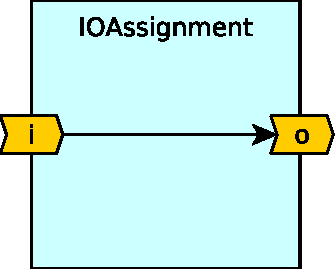
\includegraphics[height=1.8cm]{graphics/IOAssignment.pdf}\\
    \end{minipage}%
    \hfill 
    \begin{minipage}[c][2cm]{0.27\textwidth}
      A single line arrow indicates a dataflow dependency \textbf{without} affecting initial conditions of the consumer.
    \end{minipage} 
    \\ 
    \hline
    \begin{minipage}{0.1\textwidth}
      \flushleft
      Directionality \\and\\ Commutativity
    \end{minipage} 
    &
    \begin{minipage}[c][1.5cm]{0.42\textwidth}
      The operator is commutative, meaning \code{a <> b} is equivalent to \code{b <> a}. One argument is the \emph{producer}, while the other is the \emph{consumer}. The dataflow direction is sensitive to the context in which the operator is applied.
    \end{minipage} 
    &  
    \begin{minipage}[c][1.5cm]{0.42\textwidth}
      The operator is non-commutative, meaning \code{a := b} determines that \code{b} is the \emph{producer}, transferring data to the \emph{consumer} \code{a}.
    \end{minipage} 
    \\ 
    \hline
    \begin{minipage}{0.1\textwidth}
      Initialization
    \end{minipage} 
    &
    \begin{minipage}[c][1.2cm]{0.42\textwidth}
      Initialization is transferred to the consumer. If the consumer has both initialization via \code{.init} and connection, then the \code{.init} is the one that takes effect.
    \end{minipage} 
    &  
    \begin{minipage}[c][1.2cm]{0.42\textwidth}
      The consumer initialization is \textbf{not} affected.
    \end{minipage} 
    \\ 
    \hline
    \begin{minipage}{0.1\textwidth}
      \flushleft
      Mutation
    \end{minipage} 
    &
    \begin{minipage}[c][0.5cm]{0.42\textwidth}
      A consumer can only be connected once at each bit.
    \end{minipage} 
    &  
    \begin{minipage}[c][0.5cm]{0.42\textwidth}
      The same bit in a consumer can be assigned to 
    \end{minipage} 
    \\ 
    \hline
    \begin{minipage}{0.1\textwidth}
      \flushleft
      Statement Order
    \end{minipage} 
    &
    \begin{minipage}[c][0.8cm]{0.42\textwidth}
      Connections statements can be placed in any order. Connection from assigned variable TBD 
    \end{minipage} 
    &  
    \begin{minipage}[c][0.8cm]{0.42\textwidth}
      TBD.
    \end{minipage}% 
    \\ 
    \hline
  \end{tabular}% 
\end{table*}



%\subsection{Simulation Constructs}
%\label{sec:simulation}
%Unlike VHDL and Verilog which were developed for simulation and only later adopted for synthesis, DFiant was developed with a synthesizable language focus in mind. Nonetheless, to test our designs we added some basic simulation-only constructs, and to clearly separate them from the rest of the language, we placed them under a separate name space -- \code{sim}. Furthermore, all simulation constructs exist only within a simulation context which is formed only if the toplevel design is actually a simulation design, \code{DFSimulation}. The \code{DFSimulation} construct typically holds both the device-under-test (DUT) and the testing logic. Currently, the DFiant compiler only supports a handful of dedicated simulation constructs.
%%\code{sim.assert} to print errors if a condition is not satisfied; \code{sim.report} for printing messages; and finally \code{sim.finish} to finish the simulation. 
%\fig{fig:FibTest} demonstrates basic testing methods in DFiant, like using \code{.prev} to inject token sequences(lines 2,3,5) and easily constructing strings via string interpolation (line 6).
%
%\begin{figure}[h]
%  \centering
%  \captionsetup{justification=centering}    
%  
%  \begin{minted}[xleftmargin=0.08\linewidth, xrightmargin=0.08\linewidth,frame=single,autogobble,linenos,tabsize=2,fontfamily=courier,fontsize=\fontsize{7}{8}\selectfont]{scala}
%	trait SeqDetTest extends DFSimulator {
%		val TestSeq = Seq(1, 1, 0, 1, 0, 0, 1, 0, 1)
%		val seqIn = DFBool() init TestSeq.reverse
%		val dut = new SeqDet {}
%		dut.seqIn <> seqIn.prev(TestSeq.length)
%		sim.report(dfs"det: ${dut.detOut}")
%	}
%  \end{minted}
%  \captionof{figure}{Simulation wrapper for our sequence detector \\ }
%  \label{fig:FibTest}
%\end{figure}






%+ C has no clear input/output notation. Input array and output array are the same.
%
%+ IDE: Intellisense, error highlighting, code completion, watches, println.
%+ Unified compilation
%+ Complete project build with the IDE. Compile results.
%Yes abstract away pipelining. No to scheduling control.
%
%Features we don't want
%simulations constructs.
%separate constraints file.
%
%VHDL Possible race conditions.
%
%
%+Include a summary table of RTL feature abstraction and how their are defined in DFiant.

